\subsection{Node analysis for $t\geq0$ - forced solution $v_6(t)$}

To complete the solution of the system, the forced solution needs to be determined. That was done using the nodal analysis method equivalent to \ref{eqnodos} but adding the current flowing thought the capacitor and changing the voltage source to it's new function ($V_s(t)=sin(2\pi f t)$ , $t\geq0$) resulting in the change of only this 3 equations.

\begin{equation}
    \begin{cases}
        V_1 - V_4 = -i e^{i 2\pi f C t} \hspace{15px} \text{(independent voltage source)}\\
        (V_5-V_2)G_3 + (V_5-V_4)G_4 + (V_5-V_6)G_5 + (V_8-V_7)G_7 + (V_8-V_6)i 2\pi f C = 0 \hspace{15px}\text{(supernodal equation)}\\
        (V_6-V_5)G_5 + (V_2-V_5)K_b + (V_6-V_8)i 2\pi f C = 0 \hspace{15px}\text{(node 6)}\\
    \end{cases}
\end{equation}

Note that the the complex phasors are being used instead of the normal sine function in order to obtain the complex amplitudes. Converting this system of equations to its matricial form, one can obtain:

\begin{equation}
\scalemath{0.8}{
    \begin{bmatrix}
     1 &  0      &  0 &    -1  &     0      &  0  &  0    &  0\\
     -G_1 & G_1+G_2+G_3 & -G_2  & 0   &  -G_3       &  0  &  0    &  0\\
     0   & -G_2-K_b    & G_2  & 0   &   K_b       &  0  &  0    &  0\\
     0   & 0        & 0   & 1 & 0       &  0  & 0   & 0\\
     0   & -G_3      &  0 &  -G_4  &   G_3+G_4+G_5 & -G_5-i 2\pi f C &  -G_7    & G_7+i 2\pi f C\\
     0   & K_b       & 0  &  0    & -G_5-K_b     & G_5+i 2\pi f C  & 0     &  -i 2\pi f C\\
     0   & 0        & 0  & -G_6   &  0         & 0   & G_6+G_7 & -G_7\\
     0   & 0        & 0  &  -K_dG_6    &  1         & 0   & K_dG_6     & -1
    \end{bmatrix} 
    \begin{bmatrix}
       V_1\\
        V_2\\
        V_3\\
        V_4\\
        V_5\\
        V_6\\
        V_7\\
        V_8
    \end{bmatrix}
    =
    \begin{bmatrix}
        -i e^{i 2\pi f C t}\\
        0\\
        0\\
        0\\
        0\\
        0\\
        0\\
        0
    \end{bmatrix}}
\label{eqnodos_forced}
\end{equation}

With the matrix defined, a program in octave was used to solve the system symbolically, to which was then substituted the frequency for $1000 Hz$ and, in order to obtain the complex amplitude, time for $0$, obtaining the values in Tab. \ref{tab:amplitude}.

The information that these complex amplitudes contain is the phase and amplitude of the oscillation, in this case forced, values that can be obtained through the complex amplitude norm and its argument, respectively, as it was done and the results are presented in Tab. \ref{tab:amplitude}.


\begin{table}[H]
    \begin{minipage}{.5\textwidth}
      \centering
      \begin{tabular}{c|c}
        \hline
     Node &  Complex Amplitude (v)\\ 
     \hline
    V(1) & -0.000000 + i(-1.000000)\\ V(2) & 0.000000 + i(-0.944378)\\ V(3) & -0.000000 + i(-0.827738)\\ V(5) & 0.000000 + i(-0.952375)\\ V(6) & -0.086752 + i(0.542623)\\ V(7) & 0.000000 + i(0.364103)\\ V(8) & 0.000000 + i(0.547147)\\ 
    \hline
      \end{tabular}
    \end{minipage}
    \begin{minipage}{.5\textwidth}
      \centering
      \begin{tabular}{c|c|c}
        \hline
          Node &  Amplitude (V) & Phase (rad)\\
          \hline
          V(1) & 1.000000 & -1.570796\\ 
V(2) & 0.944378 & -1.570796\\ 
V(3) & 0.827738 & -1.570796\\ 
V(5) & 0.952375 & -1.570796\\ 
V(6) & 0.549514 & 1.729330\\ 
V(7) & 0.364103 & 1.570796\\ 
V(8) & 0.547147 & 1.570796\\ 

          \hline
      \end{tabular}
    \end{minipage}
    \caption{Amplitudes for the forced solution osculations}
    \label{tab:amplitude}
\end{table}

With this information the forced solution can be plotted, in specific, in Fig.\ref{fig:forced}.

\begin{figure}[H]
    \centering
    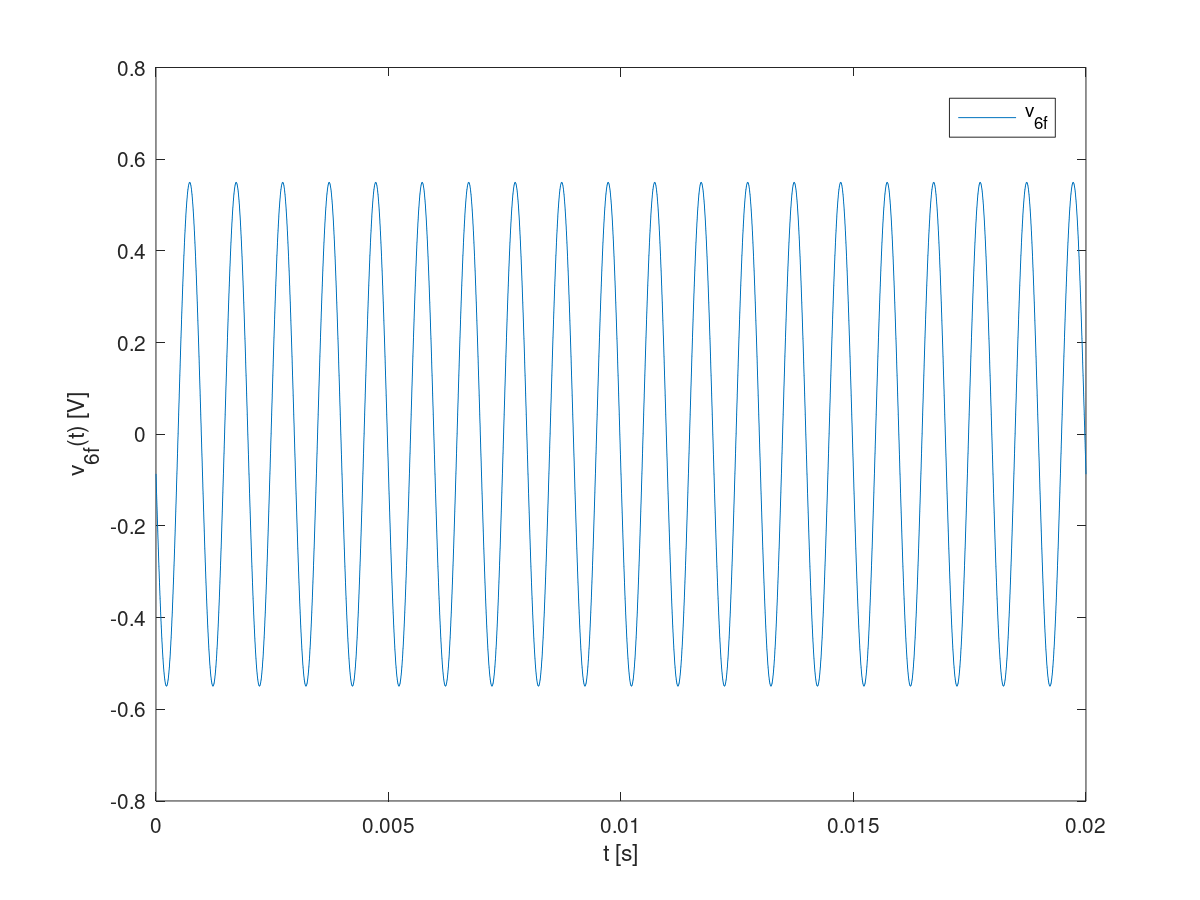
\includegraphics[width = 0.85\linewidth]{../mat/v6f.png}
        \caption{\textit{Plot of the forced solution for the voltage on node 6 in the interval $t\in[0,20]ms$ as shown on the plot}}
    \label{fig:forced}
\end{figure}

With both natural, obtained in Fig. \ref{fig:natural} and forced solutions, obtained in Fig. \ref{fig:forced} determined it's easy to add the 2 in order to obtain the complete solution, which for $V_6(t)$ is ploted in Fig. \ref{fig:complete}

\begin{figure}[H]
    \centering
    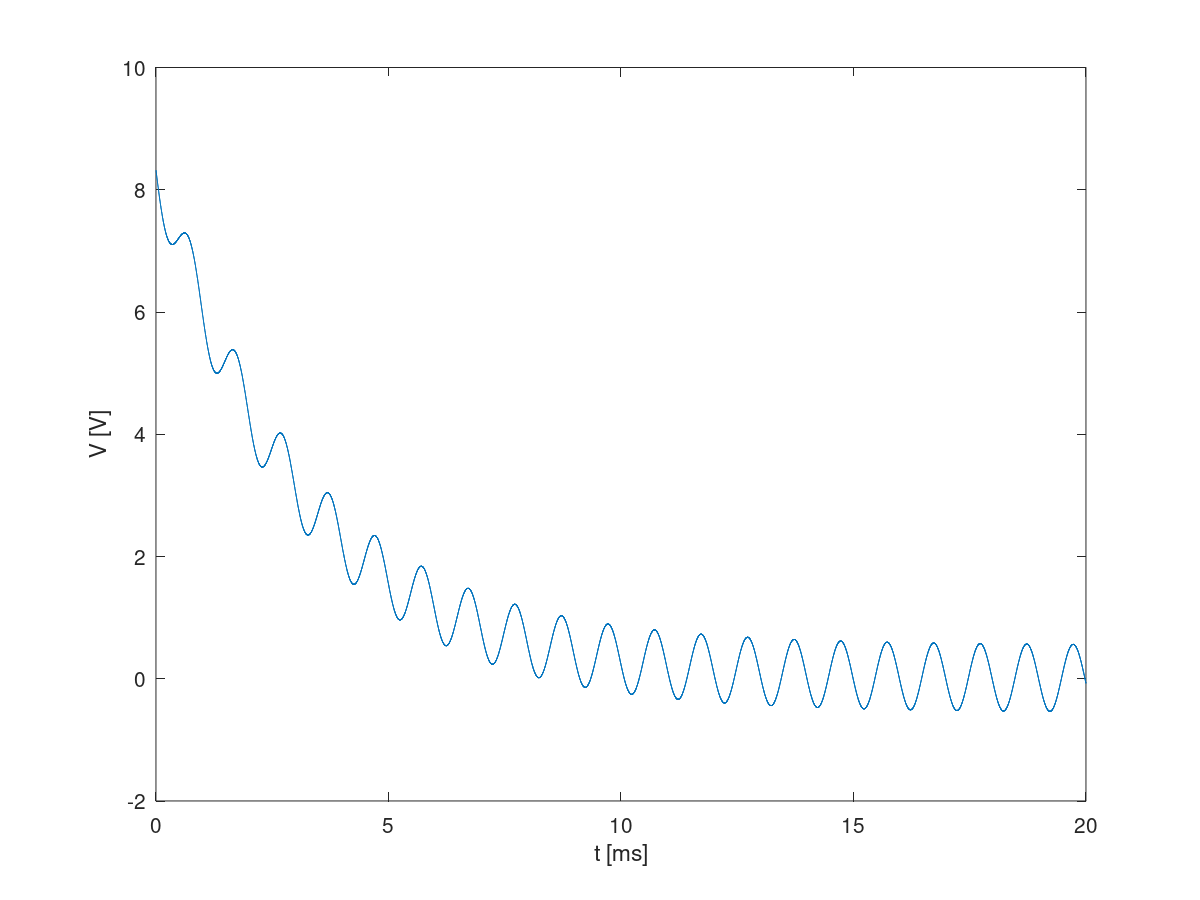
\includegraphics[width = 0.85\linewidth]{../mat/v6fn.png}
        \caption{\textit{Plot of the complete solution for the voltage on node 6 in the interval $t\in[0,20]ms$ as shown on the plot}}
    \label{fig:complete}
\end{figure}

For further understanding the behaving of the system, the voltage in node 6 and the input voltage can both be ploted for before and after $t=0$, by merging the results from the previous theoretical analysis, resulting in what is seen in Fig. \ref{fig:tudo}.

\begin{figure}[H]
    \centering
    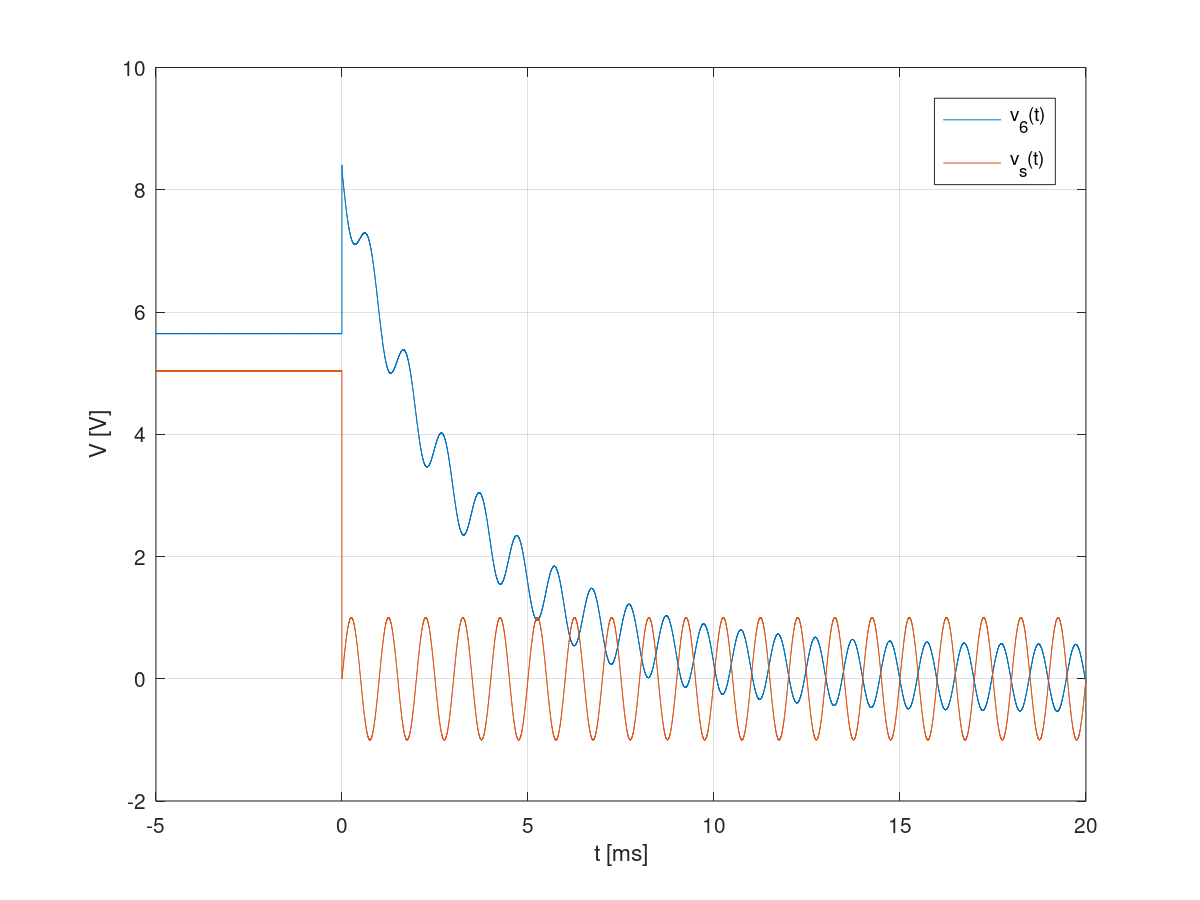
\includegraphics[width = 0.85\linewidth]{../mat/v6totsze.png}
        \caption{\textit{Plot of the complete solution for the voltage on node 6 and the input voltage  in the interval $t\in[-5,20]ms$ as shown on the plot}}
    \label{fig:tudo}
\end{figure}

As expected we can see that the discontinuity in the voltage source causes a discontinuity in the voltage in node 6, just not as intense and the system takes some time to reach the equilibrium and adapt to a behavior similar to its source. It's also notable that these 2 voltages are separated in phase by half a period.
